\section{Background}
\subsection{Neural Network}
\dmcmt{There was some general definitions of what an nn is in this section,
removed for now, nor really necessary, maybe can add a notation section if at
all necessary}

\subsection{ Formal Analysis of Neural Networks }
\dmcmt{This section used to be titled Neural Network Verification, and explained
    the general idea of neural net verif, and some stuff on prop encoding. We
    are not doing exclusively verif. So, some more general and shorter
    discussion on formal analysis of nn added.}

Several techniques and methods have been studied to improve the reliability and
trustworthiness of \dnn deployed in safety critical settings via formal
analysis. This includes verifying \dnn with respect to a given
safety property \cite{reluplex, cegar-nn, deeppoly, cegarette, cleverest-nn,
conv-abs-gk, deep-abstract, lin-comb-abs-jan}, providing formal explanations of
the behavior of the \dnn \cite{minimal-image-fxai, overview-fxai}, and others.
\dmcmt{Is the and others okay? Ref the backdoor attacks work?} To provide the
formal guarantees behind the analysis performed, all of these techniques rely on
making \textit{neural network queries}. 

These neural network queries are of the form $(P, \mathcal{N}, Q)$, and ask if
there is an input $x$ to $\mathcal{N}$ for which the formula $P$ holds so that
the formula $Q$ holds on the output $\mathcal{N}(x)$. While there are several
tools that can handle such queries, like \marabou and \abcrown, scalability
remains an issue.

\subsection{Counter-example guided abstraction and refinement}
\dmcmt{Again, we dont need to talk about CEGAR, exception being acasxu
experiments, so the section on cegar has been removed. Maybe have 2 lines and a
cite in acasxu exps?}

\subsection{Neural Network Abstractions with Strong Guarantees}

In this work, we focus on obtaining an abstract network \abs from a given
concrete network \cnc so that certain 

\subsection{Neural Network Splitting and Merging}
\dmcmt{Why Inc Dec? To get soundness. So, start by: to provide a strong formal
connection between \abs and \cnc, we follow the approach from
\cite{cegar-nn}. 2 diffs: 1. They focus on a safety prop, we aim to get
a general fw for any formal analysis not just safety verif. 2. We use inc-dec
only, not pos neg. That is sound because we can re-merge pos and neg versions
without changing behavior, since input weights are same, and max/min merge from
\cite{cegar-nn} doesn't depend on pos/neg.
Algos, diags unnecessary.
}

\dmcmt{Do we need to add a reference for 2-class?}

To transform \cnc into \abs 


\subsubsection{Increment Decrement Splitting}
To aid in the process of constructing such an over-approximate network 
we begin with the creation of an equivalent network, denoted as $\mathcal{N}'$,
 ensuring that $\mathcal{N'}(x)$ equals $\mathcal{N}(x)$ for all $x$.
To build this equivalent network, we perform an `Increment/Decrement'
splitting of neurons in our original network $\mathcal{N}$. Upon reflection, 
it became apparent to us that a two-class classification was more fitting for 
our needs, deviating from the initially recommended four-class classification 
outlined in the original work by \cite{cegar-nn}. Neurons are categorized as 
`Increment (Inc)' if increasing their values increases the output neuron's value,
 and as `Decrement (Dec)' if decreasing their values achieves the same result.

\begin{algorithm}[H]
    \caption{split\_Inc\_Dec}
    \begin{algorithmic}[1]
        \State Initialize M, the set of nodes that are marked, to \{out\_node\} and mark out\_node as \textbf{Inc}.
        \State Let $R$ be the set of nodes with successors in $M$.
        \State Define $\text{sign(u,v)}$ as the sign of the weight from the node $u$ to $v$.
        \State Define $\text{Class(v)}$ as $1$ when $v$ is marked as $\textbf{Inc}$, and $-1$ otherwise.
        \While {\text{node} $\notin M$ and node $\notin$ input\_nodes}
        \State Pick a node $u$ such that $u \in R-M$
        \State Suppose $u$ feeds into $x_1,x_2,x_3,..$ and $y_1,y_2,y_3..$ where $\text{sign($u,x_i$)} = \text{Class($x_i$)}$ for all $x_i$, $\text{sign($u,y_i$)} \neq \text{Class($y_i$)}$ for all $y_i$.
        \State Split $u$ to $u_1$ and $u_2$, where $u_1$ feeds into all the $x_i$ and $u_2$ feeds into all the $y_i$.
        \State Mark $u_1$ as \textbf{Inc} and $u_2$ as \textbf{Dec}
        \State Insert $u_1$ and $u_2$ into $M$ and their predecessors into $R$
        \EndWhile
        \end{algorithmic}
\end{algorithm}


\subsubsection{Abstraction}
\dmcmt{This is not much different from what \cite{cegar-nn} does, so we can say
    as much and push it into prev secion. Previous section can be titled
splitting and mergign for ensuring soundness or something}

\begin{figure}[H]
    \centering
    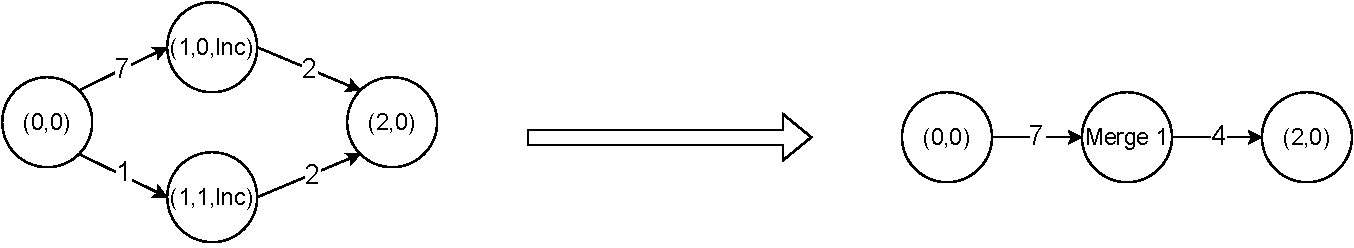
\includegraphics[width=0.5\textwidth]{diagrams/Abstraction_part1.pdf}
    \caption{Merging of Increment Neurons}
    \label{Figure: Merge1}
    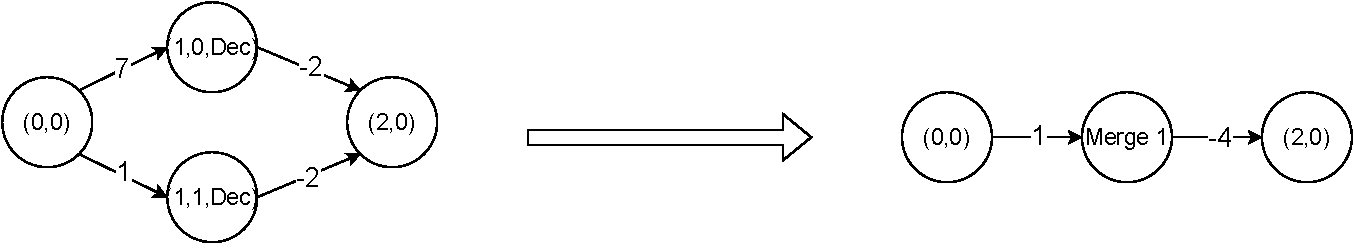
\includegraphics[width=0.5\textwidth]{diagrams/Abstraction_part2.pdf}
    \caption{Merging of Decrement Neurons}
    \label{Figure: Merge2}

\end{figure} 
The increment/decrement splitting of the neural network $\mathcal{N}$ to 
the new network $\mathcal{N'}$ changes the structure of the neural network but
 does not change the value of the output neuron. If we want to construct
  a neural network $\mathcal{N}''$ which over-approximates the value of 
  the original network $\mathcal{N}$ i.e $\forall x \in X, \hspace{1mm} 
  \mathcal{N''}(x) \geq \mathcal{N}(x)$, then we perform the following steps:
\begin{enumerate}
    \item When merging two $\textit{Increment Neurons}$, discard one of those neurons and replace the incoming weight by maximum of all the incoming weights and the outgoing weight by summation of all the outgoing weights. 
    \item When merging two $\textit{Decrement Neurons}$, discard one of those neurons and replace the incoming weight by minimum of all the incoming weights and the outgoing weight by summation of all the outgoing weights. 
\end{enumerate}


\subsection{Refinement }
\dmcmt{This section should re-frame what gk's refinement does beyond cegar/verif
    into a more general fw. Then, it should point out the deficiencies (pulling
    out one neuron, singleton nodes, etc.) in this refinement approach and
    motivate the partial order. 
}

\dmcmt{    Do we talk about singleton nodes in intro or abstract? We were doing
    this in prev version
}

After merging the neurons, we introduce an over-approximation into 
the new network $\mathcal{N''}$. And since $\mathcal{N''}(x) \geq \mathcal{N}(x)$,
 there might exist a $x$, for which, $\exists x \in X, \hspace{1mm} \mathcal{N''}(x)
\geq c$ but $\nexists x \in X, \hspace{1mm} \mathcal{N}(x) \geq c$. 
Therefore, if a counter-example `$\beta$' returned is not a valid counter-example,
which means, $\mathcal{N''}(\beta) \geq c > \mathcal{N}(\beta)$, then, we must 
reverse some of the merges performed previously to get a new network which mitigates
the extent of the over-approximation for us to get a valid counter-example or to 
prove that the original property is valid.

In \cite{cegar-nn}, the authors employed a Counterexample-Guided Abstraction 
Refinement (CEGAR) approach to eliminate the spurious counter-examples. 
They utilized a counter-example ($\beta$) to identify a neuron $n_{(i, j)}$ 
that had been merged into the node `$r$' for refinement. The authors then 
computed the value $\omega$ which was equal to 
$|v_i^j(\beta) - r(\beta)| \cdot |w_{n_{(i-1, k)},n_{(i,j)}}-w_{n_{i-1,k},r}|$, 
where $v_{(i, j)}(\beta)$ denotes the value of $n_{(i, j)}$ at the 
counter-example $\beta$, $r(\beta)$ denotes the value of the 
representative neuron $r$ at the counter-example $\beta$, $w_{n_{(i-1,k)},n_{(i,j)}}$ 
denotes the weight between a neuron $n_{i-1,k}$ and a neuron $n_{i,j}$. 
If this value $\omega$ was over a recommended amount $\epsilon$, they proceeded to 
separate $n_{(i, j)}$ from $r$ to potentially eliminate the spurious counter-example 
$\beta$.

\dmcmt{ 
    An example of Elboher's Refinement where we get a lot of singletons
}


 In the next section, we present a new method for merging neurons in 
 order to reduce the number of refinement steps, thereby expediting the 
 verification process.
